\fontsize{12}{12}\selectfont
\chapter{Selecci�n de la herramienta para Data Discovery}
Fue analizado el Cuadrante M�gico de Gartner[REF] para la selecci�n de la mejor herramienta que se adecue a los criterios necesarios para ser utilizado en esta tesis.

\textsc{\begin{figure}[H]
	\centering
	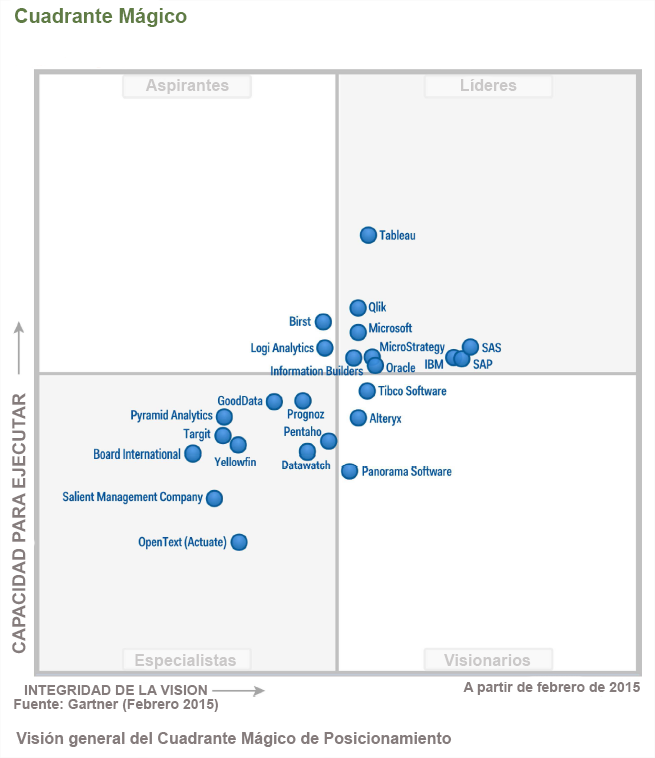
\includegraphics[width=160mm]{Magic-Quadrant.png}
	\caption{Cuadrante M�gico para BI y Plataformas Anal�ticas}
	\label{fig:magicQuadrant}
\end{figure}}


Tableau tiene una posici�n fuerte en capacidad de ejecuci�n en el eje de l�deres del cuadrante. La herramienta Tableau fue la que mejor se adecu� a las necesidades del trabajo de Tesis, dado que cuenta con una versi�n P�blica para la construcci�n y publicaci�n de dashboards, adem�s de la facilidad de uso que nos proporciona. Tableau Desktop, la cual se basa en tecnolog�a drag and drop (arrastrar y soltar) permite analizar datos r�pidamente y le permite ver los cambios en tiempo real sin necesidad de codificaci�n.


\begin{figure}
\centering
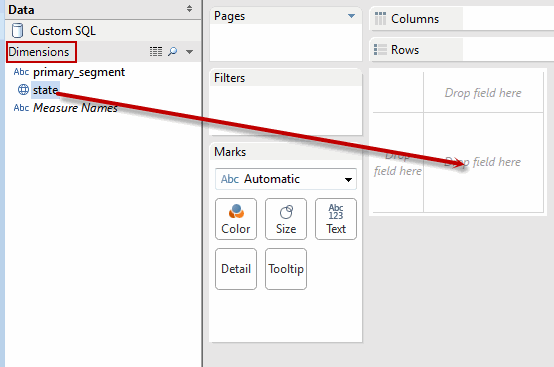
\includegraphics[width=0.7\linewidth]{tableauDragAndDrop.png}
\caption{}
\label{fig:tableauDragAndDrop}
\end{figure}
%
%
%\textsc{\begin{figure}
%	\centering
%	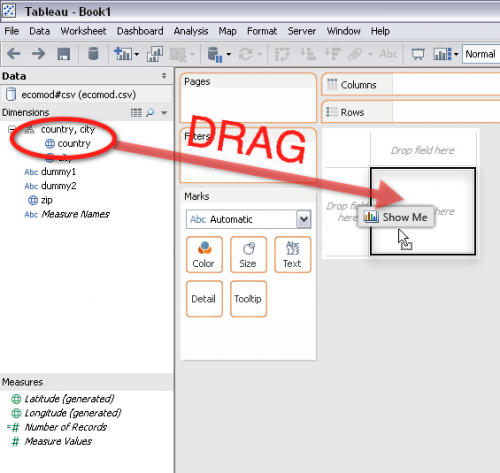
\includegraphics[width=0.7\linewidth]{figuras/tableauDragAndDrop2}
%	\caption{}
%	\label{fig:tableauDragAndDrop2}
%\end{figure}}
%
%
%
%\textsc{\begin{figure}
%	\centering
%	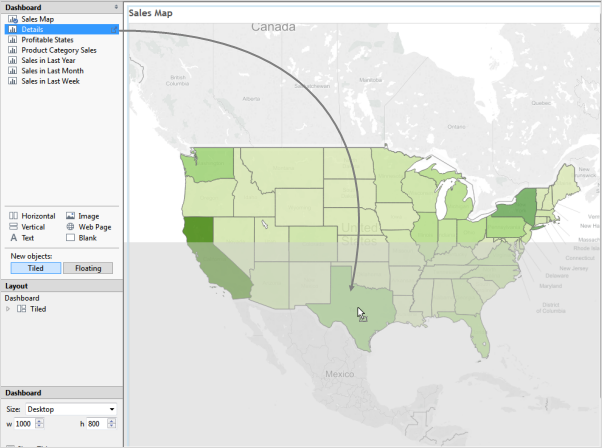
\includegraphics[width=0.7\linewidth]{figuras/tableauDragAndDrop1}
%	\caption{}
%	\label{fig:tableauDragAndDrop1}
%\end{figure}}